\section{Related Work}\label{section2}
Each node with a packet to transmit must join a contention for the channel. In CSMA/CA, nodes are deferred for a fixed period of idle-channel time and then for a random backoff period before attempting transmission. Because it only considers a single kind of traffic, the default contention parameters are the same for all contenders. 

In this section we present the traffic differentiation capabilities of EDCA as well as other enhancements proposed by the research community.

\subsection{Enhanced Distributed Channel Access}\label{EDCA}
EDCA provides traffic differentiation by defining three parameters for each of the four ACs. First, by adjusting the Transmission Opportunity (TXOP) an AC may transmit several packets without repeating the contention for the channel, thus achieving greater throughput than other ACs. The other two parameters are related to the contention process, namely the Contention Window (CW$_{\min}$ and CW$_{\max}$, for minimum and maximum respectively) and the Arbitration Inter-Frame Spacing (AIFS). The contention windows limit the random backoff period, while the AIFS defines the fixed waiting period when the channel is idle. ACs with low contention windows and short AIFS will access the channel quicker, that is, have higher priority.

WLANs time is slotted. That is, it is composed of tiny empty slots of fixed duration $\sigma_{e}$, collisions and successful slots (which contain collisions or a successful transmission. Their duration denoted by $\sigma_{c}$ and $\sigma_{s}$, respectively)\footnote{Empty slots are much shorter than collision or successful slots, that is, $\sigma_{e}\ll\min(\sigma_{c},\sigma_{s})$.}. DCF instructs backlogged stations to wait for a random number of empty slots (random backoff period) before attempting transmission.

EDCA extends directly from DCF. In its place, EDCA declares up to four Access Categories (AC), each one an instance of DCF with different contention parameters that allow a statistical prioritisation among them~\cite{perahia2013next}. Traffic types, declared by the IEEE 802.1D standard~\cite{8021d} are then mapped to the four ACs in EDCA (MAC bridging). The mapping is shown in Table~\ref{tab:prioritiesMap}.

	\begin{table}[t]
		\centering
		\caption{AC relative priorities and mapping from 802.1D user priorities (extracted from~\cite{perahia2013next})}
		\label{tab:prioritiesMap}
		\begin{tabular}{|c|c|c|c|}
			\hline
			{\bfseries Priority} & {\bfseries 802.1D User priority} & {\bfseries AC} & {\bfseries Designation}\\
			\hline
			\multirow{2}{*}{Lowest} & 1 & \multirow{2}{*}{BK} & \multirow{2}{*}{Background}\\
			\cline{2-2}
							     & 2 &				    &\\
			\hline
			\multirow{2}{*}{}	     & 0 & \multirow{2}{*}{BE} & \multirow{2}{*}{Best Effort}\\
			\cline{2-2}
							     & 3 & 				     &\\
			\hline
			\multirow{2}{*}{}	     & 4 & \multirow{2}{*}{VI} & \multirow{2}{*}{Video}\\
			\cline{2-2}
							     & 5 & 				     &\\
			\hline
			\multirow{2}{*}{Highest}& 6 & \multirow{2}{*}{VO} & \multirow{2}{*}{Voice}\\
			\cline{2-2}
							     & 7 & 				     &\\
			\hline			
		\end{tabular}
	\end{table}
	
Every backlogged AC joins the contention for the channel by drawing a random backoff, $B[\text{AC}]\leftarrow\mathcal{U}[0,CW_{\min}[\text{AC}]-1]$; where $CW_{\min}[\text{AC}]$ is the minimum contention window for said AC. Each AC waits for a fixed $AIFS[\text{AC}]=SIFS\footnote{The Short Inter-Frame Space (SIFS) is defined in~\cite{802Standards}. It is equal to 10 or 16$\mu$s for 802.11 n and ac respectively.}+\sigma_{e}(AIFSN[\text{AC}]-1)$ period of inactivity in the channel and then starts decrementing its random backoff. Each passing empty slot decrements $B[\text{AC}]$ in one. When the backoff counter expires ($B[\text{AC}] = 0$), the AC will attempt transmission. Table~\ref{tab:EDCAparams} shows the default CW, AIFSN and TXOP values specified for EDCA. 

	\begin{table}[t]
		\centering
		\caption{Deafult EDCA parameters (extracted from~\cite{perahia2013next})}
		\label{tab:EDCAparams}
		\begin{tabular}{|c|c|c|c|c|c|}
			\hline
			{\bfseries AC} & {\bfseries CW$_{\min}$} & {\bfseries CW$_{\max}$} &		{\bfseries m}		& {\bfseries AIFSN} & {\bfseries TXOP limit}\\
			\hline
			BK 		       & 		32			&		1024		   &			5			& 		8		  &		0 (only one MSDU)\\
			%\hline
			BE 		       & 		32			&		1024		   &			5			& 		4		  &		0 (only one MSDU)	\\
			%\hline
			VI 		       & 		16			&		32		  	   &			1			& 		3		  &		3.008 ms		\\
			%\hline
			VO 		       & 		8			&		16		  	   &			1			& 		3		  &		1.504 ms		\\
			%\hline
			Legacy	       & 		16			&		1024	  	   &			5			& 		3		  &		0 (only one MSDU)\\
			\hline
		\end{tabular}
	\end{table}

As it can be observed in Table~\ref{tab:EDCAparams}, ACs BK and BE may only send one MAC Service Data Unit (MSDU) upon each attempt. Whereas VI and VO can allocate the channel for longer periods. The TXOP parameter offers resource fairness rather than throughput fairness, that is, all ACs of the same category will receive close to the same average channel time regardless of its data rate. Furthermore, because the CW and AIFSN values for VI and VO are smaller than the others, on average these ACs will access the channel quicker; thus providing priority in the contention. The relative AIFSN lengths for each AC are shown in Fig.~\ref{fig:AIFSN}.

	\begin{figure}[t]
	\centering
		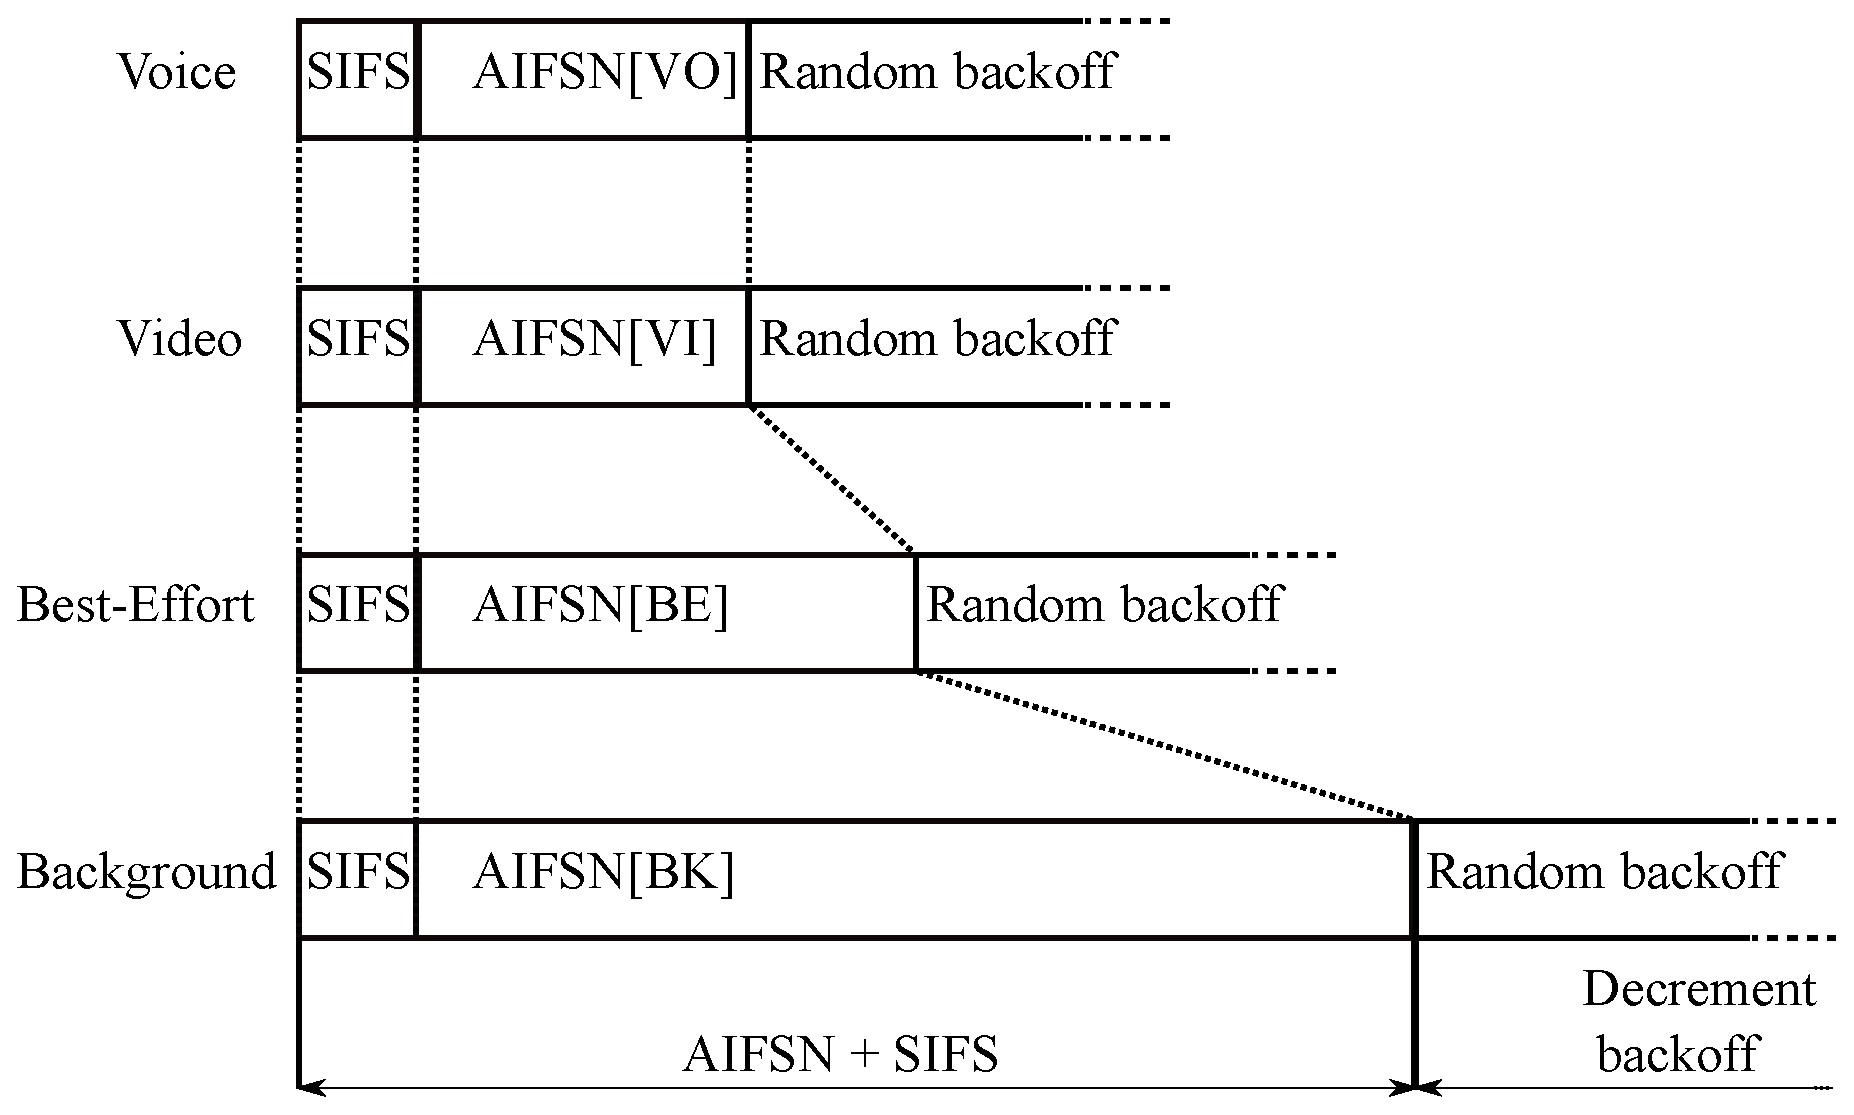
\includegraphics[width=\linewidth]{figures/AIFSN.eps}
		\caption{AIFSN values for each AC. From lowest (BK) to highest priority (VO).}
		\label{fig:AIFSN}
	\end{figure}

While being effective in providing traffic differentiation and priority, in principle EDCA is unable to eliminate collisions. For instance, two ACs from different contenders may draw the same random backoff and consequently attempt transmission in the same time slot, causing a collision. Collisions force a retransmission of the frame by repeating a contention after doubling the current CW. Furthermore, if two or more ACs within a node experience a backoff expiration at the same instant, a Virtual Collision (VC) will occur. VC are resolved by granting the channel to the highest priority AC, while doubling the CW for the lower priority ACs; just as it is done in the event of a real collision.

It follows directly from above that collisions waste channel time and thus contribute to the throughput degradation in WLANs. Moreover, the probability of collision increases as more contenders join the network, each one having four ACs attempting to gain access to the channel.

\subsection{Other contributions}
Because ACs in EDCA perform contention independently of the others, each AC mimics a station. This explains why the collision probability in EDCA is higher than in single-AC DCF networks with the same number of saturated nodes. Furthermore, the contention parameters in EDCA work better in scenarios with low number of contenders, but often cause starvation of low priority ACs in crowded scenarios (see~\cite{990806} and Section~\ref{sim:results}).

Therefore, great efforts have been directed towards parameter adjustments in EDCA~\cite{throughputGuarantees,6614899,4594854}. For example, by dynamically adjusting the AIFS for each AC it is possible to maintain traffic differentiation while avoiding the starvation of low priority ACs. This is especially relevant in WLANs where all ACs are required to have effective throughput, like in~\cite{6614899}. Further, by randomising the AIFS values it is possible to increase the channel utilisation in EDCA~\cite{4594854}. Nevertheless, all these approaches either require information about the number of nodes participating in the contention, or inject additional traffic to the network, which may be unsuitable for crowded scenarios.
